% !TEX root = Hogwarts_1347.tex

\chapter{Of Crooked Chimneys and Sapphire Sparks}

The street was narrow, but the buildings on either side seemed to soar impossibly high, their architecture a riot of the medieval and the magically enhanced---gabled roofs, crooked chimneys that puffed sparks of emerald and sapphire, and windows that glittered with untold enchantments. The ground was paved with smooth, dark stone, and the crowd was a colourful mix of wizards and witches in robes of every cut and colour, interspersed with their children, some carrying cages and others clutching hefty books.

\enquote{The money, Thomas,} Alianor murmured, reaching into her purse and handing him a handful of unfamiliar, heavy coins. \enquote{Keep it safe.} The coins were Galleons---large, heavy gold pieces, round and bearing the image of a creature, alongside smaller Sickles of silver and Knuts of bronze.

As they stepped fully onto the thoroughfare, Thomas's eye was instantly drawn to a series of paper posters plastered somewhat haphazardly upon a sturdy stone wall of a building across the lane.

He froze.

The posters, with surprisingly high detail for the time, showed the image of a woman in her mid-thirties, her face etched with a mix of fierce determination and a subtle, unsettling sorrow. Her hair, like his, was blond, almost white. She was holding a wand in her left hand with an almost aggressive confidence.

The bold, stark lettering beneath her image, written in a magically indelible ink, declared a single, haunting question:

\begin{quote}
    \enquote{What happened to Mary Elizabeth Blackwood, legendary Auror of the Council?}
\end{quote}

He stared at the face. The posters around it only deepened the mystery. One proclaimed her \enquote{The Left Hand of the Wizards' Council}. Another spoke of her as a \enquote{Legendary Turney and Jousting Champion}.

A strange, prickling sensation ran across Thomas's scalp. Instinctively, he raised his left hand and passed it quickly over his bright, pale hair.

As his fingers brushed the roots, the colour {shifted}. It darkened, deepening to a shade of dark brown, a rich, earthy colour that grounded his features. At the same time, the sickly pale tone of his skin warmed, gaining a healthier, almost tanned glow. The change was swift, subtle, and profound. His piercing grey eyes, however, remained the same colour.

He looked back at his mother. Alianor, who had been watching the street, turned to him and saw the change in his hair, the intense focus on the wall, and the sudden fear in his pale eyes. She only gave a small, almost imperceptible nod.

\enquote{We move, Thomas,} she said, her voice firm. \enquote{We have much to do.}



\section*{The Scribe \& The Serpent}
 
Their first stop was a shop that seemed to vibrate with a low, thrumming energy. It was a dusty, cramped store with tall piles of worn books and scrolls. Alianor Blackwood gripped her son Thomas's shoulder protectively as they stepped over the threshold of The Scribe \& The Serpent.
 
Inside, the smell of new parchment and dust was overwhelming. A small, bespectacled witch was using her wand to lift stacks of heavy, leather-bound books and organise them onto precariously high shelves. In the corner of the shop, enchanted feathers, moving on their own, meticulously copied texts from old scrolls onto fresh, cream-coloured parchments. As soon as the script was complete, the newly inscribed parchments neatly folded themselves and began to stack with perfect precision. A charmed, silver needle then danced into motion, expertly sewing the stacked parchments together along one edge, seamlessly forming the gathered pages that would become the core of a new book. With a rustle of displaced air, robust hard covers then flew from a nearby shelf to join the newly sewn pages. They were built for permanence: thick wooden boards, often oak or beech, were covered in sturdy leather like pigskin or calfskin. Their binding was a heavy-duty affair, as they were sewn directly onto leather thongs or cords that were firmly attached to the boards. Practical, decorative metal fittings --- clasps, corner pieces, and bosses --- were frequently used to embellish them, with the result that they were made exceptionally heavy, thick, and undeniably sturdier than most contemporary covers.
 
The shopkeeper, whose beard looked woven from cobwebs, scraped a stool back.
 
\enquote{We require the first-year books for Hogwarts,} Alianor said, smoothing her simple wool gown. She produced a rolled parchment from her satchel and unfurled it with a practised snap.

\begin{figure}[bt]
    \centering
    %\raggedleft
    %\hspace*{8cm}
    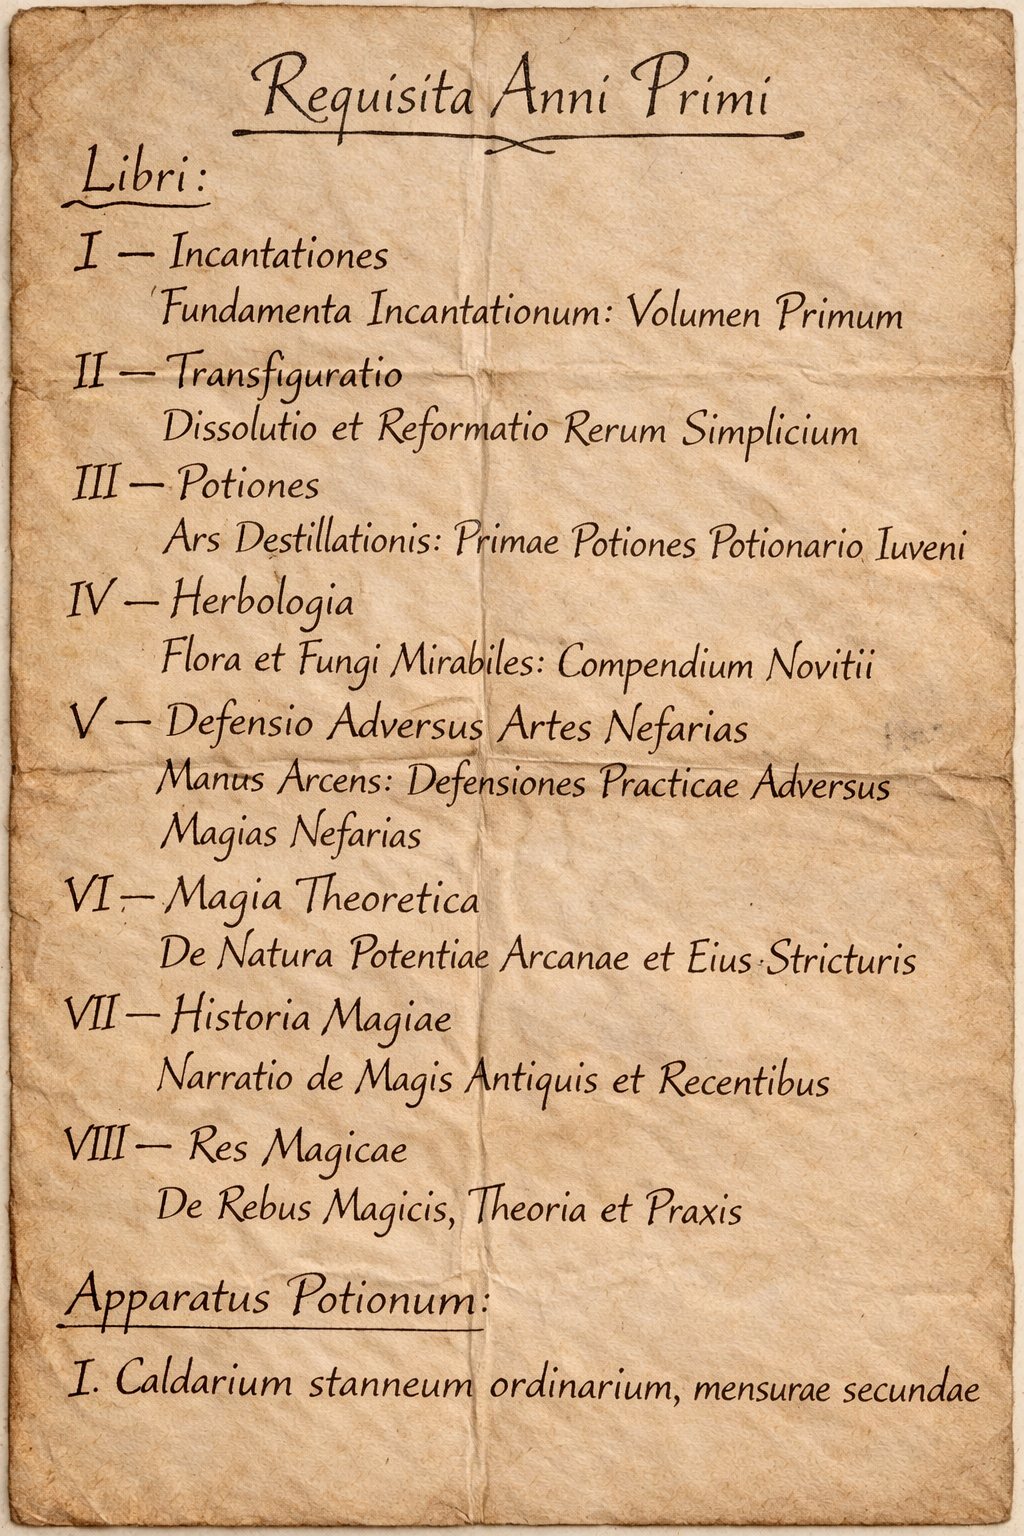
\includegraphics[width=0.5\textwidth]{images/fig_requisita_anni_primi.png}
    %\caption{The hare}
    \label{fig:hare}
\end{figure}
 
\enquote{Very well,} the shopkeeper croaked, barely looking up.
 
Alianor read from the top of the list: \enquote{For Charms: \textit{Fundamenta Incantationum: Volumen Primum} --- Foundations of Enchantment: Volume I.}
 
The shopkeeper grunted, shuffled over to a back shelf, and returned with a formidable leather-and-wood volume edged with protective silver-leaf. \enquote{This is the one your son will spend most time with,} he said, setting it down on the counter. \enquote{Basic levitation and illumination, nothing too strenuous.}
 
Alianor nodded, running a thumb over the cold metal. She glanced back at her parchment. \enquote{For Transfiguration: \textit{Dissolutio et Reformatio Rerum Simplicium} --- The Unmaking and Remaking of Simple Things.}
 
The shopkeeper set down a massive, scarred volume. \enquote{Dragon hide binding, that one. Very durable. Focuses mostly on turning one simple, small object into another.}
 
Thomas, eyes wide, whispered, \enquote{Like turning a feather into a pin?}
 
\enquote{Exactly so, boy,} the shopkeeper confirmed.
 
Alianor read the next title from her list. The shopkeeper shuffled to the back and returned with another volume. She read another. He fetched another. And another.
 
Thomas watched the tower of knowledge grow on the counter with mounting apprehension. Potions. Herbology. Defence Against the Dark Arts. Theoretical Magic. History of Magic. Each book was heavier than the last, each title longer and more intimidating than the one before it. He tried to imagine carrying them all, never mind reading them, never mind understanding them, and felt a quiet, sinking dread settle in his stomach. The counter groaned under the collective weight.
 
Alianor read the final title from her list: \enquote{For Magical Artefacts: \textit{De Rebus Magicis, Theoria et Praxis} --- Magical Artefacts, Theory and Practice.}
 
The shopkeeper pushed forward one last thick, heavy volume. \enquote{Covers the essence and use of common enchanted items --- wands, brooms, mirrors, that sort of thing. Crucial for understanding how many things around us work.}
 
\enquote{That seems\ldots{} extensive,} Alianor said, looking at the formidable tower of knowledge for her eleven-year-old.
 
\enquote{It is Hogwarts,} the shopkeeper sniffed. \enquote{Learning requires weight.} He paused, looking Thomas up and down with keen, narrow eyes. \enquote{The boy\ldots{} does he command the Latin tongue well?}
 
Alianor shifted her weight. \enquote{He understands it, yes.}
 
\enquote{All these texts, madam, are written in Latin, save for some footnotes. It is also the common language used to minister the courses at the school, and the basis for most spells. While the English tongue is useful in the corridors, your son will need fluent Latin to follow his Professors and understand the finer points of the magical theory and incantations. He will also need it to communicate with many of his peers, who come from all corners of the British Isles, Normandy, and even farther east. It is the language of higher learning.}
 
A small, genuine smile touched Alianor's lips. \enquote{My late husband was insistent upon it. We lived in Hogsmeade when Thomas was very young, and his father taught him to speak it almost before he could run. After his passing and our move to London, I hired him a tutor, a Master Edmund, a very good one. Thomas has a solid grasp of it, I promise you. His private library, while entirely mundane, is quite extensive for a Muggle's collection. He will not be found wanting for reading practice.}
 
The shopkeeper let out a satisfied grunt, finally accepting the situation. \enquote{Very well. A well-prepared student is a boon to the school. Now, we must gather the rest of your apparatus. You'll need a \textit{calamus scriptorius}, or a self-scribing charmed quill.}
 
He gestured to the stack of heavy books. \enquote{You'll learn all about them in your Magical Artefacts course, I suppose. But for now, know that you'll need it to copy the texts in the Hogwarts Library. Some of those manuscripts are far too delicate to be handled by a trembling young hand, and far too long to be copied by a slow one.}
 
The shopkeeper shuffled a few steps and reached into a carved wooden box lined with deep purple velvet. He withdrew a beautiful, snowy-white feather quill, fitted with a slender nib. It was decorated with small and tasteful silver ornaments woven near the base, glinting subtly in the dim light.
 
\enquote{This one,} the shopkeeper announced, holding it out for Thomas to see. \enquote{Is top-grade for a first-year. It is fluent in Latin, naturally, but also the English tongue, Celt, Scott, Irish, Norman French, and Greek --- with a clear Byzantine influence in the last one.}
 
Thomas reached for it with reverence, careful not to touch the delicate tip. It felt strangely light, yet humming with purpose.
 
Alianor tilted the box, catching the light on the silver ornaments, and raised an eyebrow at the faint price stamped beneath the velvet lining. \enquote{A charming piece,} she commented, the warmth of her tone not quite reaching her shrewd eyes. \enquote{But the cost, I fear, is even more charming. It is a steep sum for a first-year's writing instrument, enchanted or otherwise. Could you not, perhaps, offer a slight reduction for a young boy with such an extensive book list?}
 
The shopkeeper paused, considering the tower of tomes they had just bought. He stroked his woven beard, conceding a point with a slow nod. \enquote{Very well. For a student of such evident preparation, I will shave the price of one Sickle, no more. But I will include a basic, non-charmed Raven Feather quill --- for his examinations, where such charms are, naturally, strictly forbidden. And,} he reached into a drawer, producing a slender wood piece with a silver rod tip, \enquote{a silverpoint\footnote{Silverpoint — A drawing instrument consisting of a thin rod of silver set into a wooden or metal stylus. It produces fine, precise lines on prepared surfaces and was favoured by artists such as Giotto di Bondone, Pietro Cavallini, and later Leonardo da Vinci. The marks cannot be erased, demanding a confident hand.}. It is not enchanted, but it is excellent for detailed illustrations in his Herbology and Potions texts, a favourite of great Muggle artists like Giotto di Bondone and Pietro Cavallini. A little extra value, free of charge.}
 
Alianor gave a slight, satisfied smile at the concession, accepting the silverpoint and the extra quill. \enquote{A fair bargain.}
 


















\section*{Eeylops}

After leaving the bookshop, Alianor and Thomas approached their next destination: Eeylops Owl Emporium and Bestiary. As they pushed through the door, they were immediately struck by the sheer quantity and variety of owls, their cages stacked from the floor to the rafters. The air was alive with a symphony of soft cooing, sharp chirps, and the occasional dry rustle of feathers.

Thomas moved through the aisles in wonder, his eyes darting between the different species:

\begin{itemize}
    \item Barn Owls: Their distinct, heart-shaped white faces and pale plumage made them look like ghosts flickering in the dim shop light.

    \item Long-eared Owls: Slender birds that sat perfectly still, their tall head tufts giving them a look of constant, startled alertness.

    \item Little Owls: Small, compact, and fierce-looking with bright yellow eyes and mottled brown feathers, they bobbed their heads as the pair passed.

    \item Great Grey Owls: Large, imposing birds with massive, circular facial discs and piercing yellow eyes that seemed to track every movement with unnerving intelligence.
\end{itemize}

Thomas stopped, mesmerised, before a massive Eurasian Eagle-Owl. It was a titan among birds, boasting prominent ear tufts and intense, fiery orange eyes that glowed like embers. Its powerful talons gripped a heavy perch, and its mottled tawny and black feathers gave it an air of authority. Nearby, a Snowy Owl sat in stark contrast, its plumage a brilliant, speckled white that seemed to capture what little light reached the corner of the shop.

\enquote{They are magnificent, Mom,} Thomas whispered, reaching toward the Eagle-Owl's cage.

\enquote{They are,} Alianor agreed, gently pulling his hand back. \enquote{But that one in particular is far too easy to spot. It would draw every eye from London to Hogsmeade. We need something more discreet, Thomas. A Tawny Owl is a far better choice---they are the most common owls in England and Scotland, making them the perfect, inconspicuous messenger.}

The emporium keeper, a wiry man named Silas Vane, looked up from a ledger. \enquote{A wise mother you have, boy,} he said, beckoning them toward a cage near the counter. Inside sat a young Tawny Owl, its feathers a beautiful, soft mosaic of rich browns and greys, designed for perfect camouflage. \enquote{This one is young, mind you. That means he's playful and full of energy --- perhaps a bit destructive with a loose scroll or a stray quill --- but that should resolve itself with time and proper training.}

Silas opened the cage slightly, and the bird let out a melodic hoot. \enquote{He's an affectionate sort, has a marvellous recall, and he's fast,} Silas added with a wink. \enquote{Really fast.}

\enquote{Does he have a name?} Thomas asked, watching the owl tilt its head curiously.

\enquote{I've been calling him Pippin,} Silas replied. \enquote{You may change it if you like, of course.}

Thomas looked at his mother, and they both shared a rare, genuine smile. \enquote{Pippin,} Thomas repeated, the name feeling right. \enquote{I like it.}

Alianor turned to Silas, her expression shifting back to her usual shrewdness. \enquote{And the price for young Pippin?} When Silas named a sum, Alianor's eyebrow arched---it was higher than she had anticipated.

\enquote{He is a prime specimen, Mr. Vane,} she countered smoothly, \enquote{but he is also, by your own admission, quite the handful for a first-year student.} After a brief, spirited bout of bargaining, Silas finally relented with a sigh.

\enquote{Very well,} Silas grumbled, though his eyes twinkled. \enquote{I'll match your price, and I'll even include a large sack of owl treats to keep him occupied while he learns his manners.}

\section*{Slug \& Jiggers}

Leaving the bright activity of the street behind, Alianor and Thomas stepped into the dim, pungent atmosphere of the Slug \& Jiggers Apothecary. The shop was a sensory assault; a heavy, complex scent of rotted cabbage and salted fish hung in the air, punctuated by sharper, more exotic notes of crushed herbs and dried resins. From the low, timbered ceiling hung bundles of dried feathers, leathery bat wings, and long, shimmering strings of dragon liver that swayed slightly in the draft.

Shadows danced across the floor, cast by the flickering green flames of a small hearth at the back. Shelves climbed every inch of the walls, crowded with thousands of glass jars containing everything from cloudy, swirling liquids to the bright, unblinking eyes of newts.

Just inside the entrance, perched atop a velvet-covered pedestal, sat an exquisite cauldron. It was a masterpiece of craftsmanship, forged from copper, polished and with ornate porcelain handles hand-painted with delicate floral patterns and reinforced with gleaming bronze filigree around the rim. Thomas stopped in his tracks, his eyes wide with admiration.

\enquote{Wow,} he murmured, reaching out to touch the cool porcelain.

\enquote{A fine piece,} the apothecary called out. He was a stooped man with stained fingers and a smudge of silver powder on his cheek. He emerged from behind a mountain of dried roots. \enquote{But not the best choice for the rigors of Hogwarts. You'll want something that can survive a mismanaged potion or a clumsy lad's elbow.}

He reached beneath a heavy wooden counter and hauled up a far more utilitarian vessel. \enquote{A standard pewter iron cauldron, size number two. It's the requirement for the school and a much sturdier option.} He set it down with a heavy, metallic \textit{thunk}. It was made of thick, dark cast iron---plain, unadorned, and fitted with simple, sturdy stoneware handles designed for function over form.

Alianor nodded in agreement, unfurling a long roll of parchment that crinkled loudly in the quiet shop. \enquote{We shall take the iron one. We also require the rest of the list: a set of glass phials, a dozen horned slugs, porcupine quills, and a set of brass scales.}

The storekeeper turned to the massive back wall, his hands moving with practiced grace. He retrieved a set of crystal-clear phials, nesting them in straw, then scooped a handful of dried, knobby horned slugs into a small tin. He added a bundle of sharp, translucent quills and a gleaming set of brass scales, placing each item one by one into the belly of the iron cauldron.

\enquote{And the total for the lot?} Alianor asked, her hand already hovering over her coin purse.

The apothecary reached for a wooden abacus sitting on the counter. It was a sturdy frame of dark oak, with polished stone beads sliding along brass rods. He moved the beads with a rhythmic \textit{click-clack}, calculating the cost of the ingredients and the equipment with effortless speed.

\enquote{That will be seven Galleons and four Sickles,} he announced.

Alianor paused, a look of genuine surprise and pleasure softening her sharp features. The price was significantly lower than she had budgeted for. Sensing a rare moment of financial breathing room, she looked around the shelves.

\enquote{Do you happen to have an oil scented with myrrh\footnote{Myrrh — An aromatic resin from trees of the genus \textit{Commiphora}, native to Arabia and the Horn of Africa, prized since antiquity for its perfum.}?} she inquired.

The apothecary nodded and reached for a top shelf, pulling down a small, elegant ceramic flask sealed with wax. \enquote{A fine choice. It's a base of sweet almond oil, heavily scented with pure myrrh and stabilised with a touch of ambergris as a fixative. It will last a long time.}

Alianor took the flask and turned to Thomas, her expression firm but not unkind. \enquote{I want you presentable, Thomas. Clean, combed, and perfumed for your professors and colleagues. The Blackwood name shall be associated with discipline, not the smell of a stable.}

She placed the small ceramic flask into the cauldron atop the scales. With the heavy iron vessel tucked under Thomas's arm, they stepped back out into the vibrant chaos of Diagon Alley.

\section*{Ollivanders}

Finally, they stood before the shop Thomas had been anticipating, and dreading, the most. The building was old, narrower than its neighbours, and seemed to emanate a profound stillness. Over the single, dusty window, faded lettering announced: \enquote{Ollivanders, makeres of fyne wandis, sythen 382 B.C.} Ollivanders: makers of fine wands since 382 B.C.

The interior of the shop was just as Thomas had imagined: quiet, dusted with a golden, moted light, and utterly dominated by wands and its small boxes.

Hundreds of thin, square boxes were stacked meticulously from the floor to the high, shadowy ceiling on the opposite side of the counter. The air was cool, dry, and charged with an almost palpable energy.

Behind a high, polished counter stood Gilbert Ollivander, the current proprietor. He was an elderly man, sharp-eyed, with thin hair and long, calloused and strong hands that seemed to have a life independent of his body. He was carefully cataloging a piece of dark, knotty wood. He looked up, his dark eyes immediately locking onto Thomas.

Alianor stood just outside the entrance to the shop, the parchment shopping list rustling softly in her hand as she read it over again. She glanced up, taking in the antique wooden sign above the door, before her eyes drifted to the bustle of the street. A vendor across the lane was selling trunks from a canvas-covered stall. She crossed over to inspect them. Inside, Mr. Ollivander, entirely oblivious to Alianor outside, said to the boy in a dry, parchment-like rustle, \enquote{Ah, another young sorcerer, come to collect his first wand.}

\begin{comment}
Alianor stood just outside the entrance to the shop, the parchment shopping list rustling softly in her hand as she read it over again. She glanced up, taking in the antique wooden sign above the door, before her eyes drifted to the bustle of the street. Inside, Mr. Ollivander said, his voice a dry, parchment-like rustle, \enquote{Ah, another young sorcerer, come to collect his first wand.} He didn't perceive Alianor at all. She was standing perfectly still, slightly concealed by the deep shadows near the archway of the entrance, her dark cloak blending into the gloom of the corridor.
\end{comment}

The old man began pulling boxes from the towering stacks with incredible speed, their contents already seemingly known to him.

\enquote{Try this, young man. Oak, Dragon Heartstring core, twelve inches, quite supple. Do you know the \textit{Lumos} spell?}

Thomas took the wand in his left hand. It felt plain, dry, and utterly inert in his grasp. He gave it a nervous flick, attempting a basic \textit{Lumos} spell. The wand only sparked weakly, sending a plume of black smoke that smelled strongly of burnt toast straight into his face.

\enquote{No, no, definitely not,} Ollivander chuckled, waving the smoke away with a flick of his wrist.

\enquote{Perhaps\ldots{} Ebony, Unicorn Hair, ten and a half inches, surprisingly whippy. Made for a duelist, this one.}

This wand was exquisitely carved with a spiral pattern, beautiful to behold. As Thomas held it, a sudden, powerful \textit{CRACK} split the air, and a pane of glass in a nearby display case shattered outward, sending glittering shards across the floor.

\enquote{Sorry!} Thomas squeaked, dropping the dangerous piece of wood.

\enquote{It is quite alright, young man,} Ollivander said, his eyes alight with a strange, almost manic curiosity. \enquote{A strong core, but entirely the wrong vessel. This is typical. The wand chooses the wizard,} he quoted his own motto solemnly. \enquote{It is an intricate and often frustrating process.}

He made Thomas try a few more. A wand of Holly flared a harmless, icy blue light that immediately winked out. One of Yew felt strangely hot and uncomfortable, like holding a burning coal. None felt right; none clicked into place.

At that moment, Alianor stepped through the doorway, a new leather trunk of deep brown with brass fittings set down heavily at her side. Her face was serious, her red hair blazing under the shop's light.

\begin{comment}
At that moment, Alianor stepped out of the shadows, her face serious, her red hair blazing under the shop's light.
\end{comment}

\enquote{Mr. Ollivander,} she said, her voice clear and carrying. \enquote{I believe you were entrusted some years ago with the care of a wand my husband made for the boy.}

Gilbert Ollivander's eyes widened as the realisation struck him. The subtle details, the familiar aura she carried---it all snapped into place. He recognised her instantly. It had been more than ten years since he had last seen her. She was easily recognisable by her red, fiery hair and vibrant expressions, even though she had noticeably aged since their last meeting.

\enquote{Alianor\ldots{} Blackwood,} he breathed, finally recognising the famous colour of her hair and the quiet authority in her manner. \enquote{The\ldots{} the piece\ldots{} yes. It's safe. Disguised in plain sight here, among my other wands.}

He moved slowly, deliberately, to the rear of the counter. He reached high, to the top stack, and gently pulled down a single wooden box. It was completely covered in the typical identifying labels, like all those of his own wands.

Alianor gently took the box, her fingers trembling slightly, and handed it to her son. \enquote{This was made for you, Thomas. By your father.}

Thomas opened the box.

The wand inside was unlike any he had seen. It was simple, unadorned, and made of a wood he couldn't name --- it was a dark and dense hardwood, with a thick oil or wax finish. The wand's texture was hand-hewn, beautifully wonky, forming a long pyramidal shape with four sides and rounded corners. A rugged iron fitting was pressed into the wooden base, serving to secure a cotton strip intended to wrap around the young wizard's wrist.

As his fingers closed around the wood, it was as if a powerful, quiet chord had been struck deep within his chest. The wand felt like an extension of his own arm, a missing piece of himself. A wave of warm, silver light erupted from the tip, washing over the entire shop, making the hundreds of stacked boxes glow for a single, perfect instant.

\enquote{Oh, my word,} Gilbert Ollivander whispered, his hand going to his chest.

Thomas felt a rush of pure elation and, with a silent command, the wand responded perfectly, holding the light steady and bright.

\section*{The Mystery of the Wand}

\enquote{This piece that truly defies me,} Ollivander admitted, leaning on the counter, his pale eyes full of bewildered respect. \enquote{I have never ceased to study it, and yet it resists every attempt to understand its creation.}

He placed both hands flat on the counter and began his explanation, his tone becoming that of a true master craftsman.

\enquote{We wandmakers work by a principle known to all true wizards: the wand chooses the wizard.} He tapped his motto. \enquote{It is a matter of the core---Phoenix Feather, Dragon Heartstring, Unicorn Hair---bonding with the wood---Holly, Oak, Ash---to find a magical echo in the soul of the one who wields it.}

He gestured to the wand in Thomas's hand. \enquote{This wand, however, was made for you, young man. Made to fit you before you even showed the first sparks of magic. And yet\ldots{} it fits your magic like a glove.}

\enquote{But why does it defy you?} Thomas asked, his curiosity now almost as great as his excitement.

\enquote{Its loyalty,} Ollivander said, his voice dropping to a near whisper. \enquote{My own creations will resist the magic of another wizard, yes. They will feel strange, heavy, or difficult to perform complex spellwork for a non-owner. But I have tried every basic, non-verbal charm on this piece---a simple \textit{Accio}, a basic \textit{Scourgify}. It refuses me completely. It will not perform the most rudimentary spell for anyone but its owner.}

He shook his head slowly. \enquote{It resists even my most advanced attempts to guess its core. The resistance is total. I can hazard a guess that the wood is Blackthorn based on the grain and texture, but its properties are completely masked. It is utterly, absolutely loyal.}

\enquote{It is a Blackwood family tradition, I believe, Mr. Ollivander,} Alianor explained softly. \enquote{Since before the Council's founding. The line of Blackwood first wands are crafted at birth, not chosen at eleven.}

\section*{Wayfarer}

Mr. Ollivander straightened his back, a rare spark of paternal pride softening his eccentric, misty-eyed gaze. He stepped toward a corner of the shop where three brooms stood displayed on a rack of dark mahogany.

\enquote{You see, young Thomas,} he began, gesturing to the instruments, \enquote{my family has lived and breathed wandcraft for generations. The call of the wood and the core has been a family tradition, followed by my father, my grandfather before him, myself and now even by my youngest, Griffin. He is also starting at Hogwarts this year by the way, you will meet him soon. But my eldest, Ariana, saw her future in the wind rather than the spark.} He chuckled, a dry sound like rustling parchment. \enquote{She deviated from the family tradition to invest herself in the fine art of broom-making. I keep a few of her pieces here to show what an Ollivander can do when she turns her hand to flight.}

He pulled the first broom from the rack. It was sturdy, with a thick ash handle and a tail of stiff, well-bound birch twigs. Simple iron stirrups were bolted to the sides. \enquote{This is the \textit{Cumbrian Stout}. A true workhorse. It is reliable, sturdy, and exceptionally easy to master. It won't win you any races, and it isn't the most agile in a sharp turn, but it will never fail you in a storm.}

He replaced it and lifted a second broom that looked like a needle of polished oak. It was slick and slender, featuring gleaming brass foot-supports that had been polished to a mirror finish. \enquote{Now, this is the \textit{Silver Streak}. It is built for one thing: raw, unrelenting speed in a straight line. It's a bit unforgiving when it comes to sharp corners.}

Finally, he reached for the third broom, and his voice took on a tone of genuine reverence. This one was slightly shorter, the handle crafted with a subtle, ergonomic curve designed to tuck perfectly against a wizard's legs and torso. The foot supports were of polished iron, sleek yet substantial.

\enquote{This,} he whispered, \enquote{is the \textit{Wayfarer}. It is the jewel of Ariana's current collection. It represents a perfect compromise --- nearly as fast as the \textit{Streak} on the straightaway, but with an agility for sharp turns that is unmatched. More importantly,} he tapped the curved handle, \enquote{it is weighted to be handled single-handed. If you are ever in a tourney, or heaven forbid, a combat situation where you must hold a wand in your other hand, the \textit{Wayfarer} will listen to your knees and your balance more than your grip.}

Thomas reached out to touch the polished wood, his eyes shining.

\enquote{Griffin is taking a \textit{Wayfarer} to Hogwarts. This specific piece, unfortunately, has already been purchased by a client as well. But you will find others just like it, and a full selection of models, at Ariana's shop on the very edge of Diagon Alley.} Ollivander said with a wink. \enquote{Or,} he looked at Alianor, \enquote{I could arrange to have one delivered directly to the boat. He is taking one of the great hulks to Hogwarts later today, isn't he?}

\enquote{He is,} Alianor confirmed. She stepped forward, her eyes narrowing as she read the price tag affixed to the broom's handle. She reached into her leather purse, her fingers dancing over the coins Hob Fox had given her, and pulled out the required gold.

\enquote{We will take it,} she stated, handing the Galleons to Ollivander. \enquote{Have it delivered to the Hogwarts boat before departure. And please,} she added, her voice softening with a hint of nostalgia, \enquote{send my compliments to Ariana. It has been a very long time since I last saw her.}

\section*{Twilfitt and Tattings}

Leaving the wand maker to his next mark, Alianor and Thomas ducked into the warm, lint-filled air of \textit{Twilfitt and Tattings}. The shop was a whirlwind of activity. The moment they crossed the threshold, a pair of enchanted measuring tapes leaped from a mahogany counter and began snaking around Thomas's limbs, cinching his waist and spanning his shoulders with frantic energy. Nearby, a self-inking quill scratched notes onto a hovering piece of parchment with a rhythmic \textit{skritch-skritch-skritch}.

The proprietor, a flamboyant man named Master Pendergast Malkin, emerged from a forest of hanging linen and silk. Alianor didn't wait for a greeting; she unfurled her parchment list. \enquote{Three sets of plain black work robes, one pair of dragon-hide protective gloves, and one winter cloak with silver fastenings, please} she commanded.

Pendergast gave a sharp flick of his wand. A silver needle and a spool of black thread took flight, diving into a stack of pre-cut robes like a pair of hunting hawks. They zipped through the fabric, darting in and out to adjust the seams to the quill's precise measurements. As each piece was finished, it folded itself into a neat square and drifted through the air to land on the front counter, joined shortly by a pair of sturdy, pebbled-leather gloves.

The shop door chimed again, admitting a trio that stood out in the crowded room. A man in sensible Muggle woollens was accompanied by two daughters. Thomas watched them, intrigued; the father spoke in a low, melodic tone, referring to the younger girl as Celine and the elder as Cecile. Their speech was a rapid-fire language that Thomas couldn't quite follow.

A seamstress wearing a measuring rope like a scarf hurried over. \enquote{Monsieur Fournier! A pleasure to see you again. What can we do for the girls today?}

\enquote{If you please,} M. Fournier said, his French accent thick and rolling. He held up a small winter cloak and a set of robes that were clearly well-loved but slightly faded. \enquote{Can these be adjusted for Celine? And she will need one new black robe as well.} He then turned to his eldest. \enquote{For Cecile, three Hufflepuff uniform dresses and a new winter cloak.}

Thomas's eyes drifted to the back of the store, where four mannequins stood like silent sentinels, each draped in the colours of the Hogwarts houses. At this period, the \enquote{dresses} were structured as long, modest kirtles with fitted bodices and sweeping skirts.

The Hufflepuff dress was a deep, earthy yellow with charcoal-grey trim, the badger emblem embroidered subtly on the breast. Thomas looked at the other three:

\begin{itemize}
    \item Gryffindor: A bold scarlet gown with gold-threaded embroidery that seemed to shimmer like fire.

    \item Ravenclaw: A sophisticated bronze-and-blue ensemble, the fabric a rich, heavy velvet.

    \item Slytherin: A gown of emerald green with silver silk lacing up the sides, looking cold and regal.
\end{itemize}

\enquote{Hopefully,} Mr. Fournier said with a hopeful smile, \enquote{Celine will be sorted into Hufflepuff as well, so she may inherit her sister's wardrobe next year.}

Celine flashed a tight, artificial smile that fooled no one, her eyes betraying the disapproval. Thomas wondered if she was tired of hand-me-downs, or if her heart was set on the vibrant scarlet of Gryffindor, or if she already had a preference for a specific house.

Thomas turned his gaze to a second set of mannequins on the opposite wall, his stomach doing a nervous flip. He found himself staring at the Ravenclaw bronze and the Slytherin silver. His father had been a Ravenclaw, a man of wit and learning; his aunt, however, had worn the green of Slytherin. He pulled his gaze away, he preferred not to think about it.

Alianor counted out the payment, her eyes never leaving Master Pendergast until the transaction was settled. \enquote{Come, Thomas,} she said sharply.

As they stepped back out into the street, Thomas looked back one last time. Master Pendergast was already stooping over the Fourniers' worn robes, his wand out to begin the task of making the old look new again.

\section*{The Astrolabe}

They made a final, brief stop at a shop specialising in celestial instruments to acquire the remaining items on Thomas's list. Among the charts and quadrants, they purchased a heavy brass astrolabe. It was a weighty instrument consisting of a thick, circular main frame called the \textit{mater} and several interchangeable plates engraved with the stereographic projection of the heavens. Atop these sat the \textit{rete}, a skeletal, ornate metal web whose points indicated the positions of the brightest stars, allowing Thomas to calculate the time and the position of the planets by aligning the \textit{alidade}---a pivoting sighting bar---on the back. With the astrolabe, a wooden quadrant for measuring altitudes, and a sprawling vellum constellation map tucked safely away, they prepared to leave.